\chapter{Background and Related Work}
% 1) Introductory paragraph: Very briefly: What is the problem and
%         why is it relevant to the audience attending *THIS CONFERENCE*?
%         Moreover, why is the problem hard, and what is your solution?
%         You must be brief here. This forces you to boil down your
%         contribution to its bare essence and communicate it directly.

In this section we lay the groundwork for describing the MacroLab
macroprogramming framework and MDB debugger and present macroprogramming and
debugging approaches similar to ours. We also describe the work related to the
various components behind occupant-oriented room-level zoning.

\section{Macroprogramming Cyber-Physical Systems}
MacroLab is an imperative vector-based macroprogramming abstraction that permits
deployment-specific code decomposition (DSCD) while MDB is the first debugger
that allows the user to navigate and view the distributed state of a program in
terms of high-level macroprogramming abstractions. In the following two subsections, we describe
the fundamentals of macroprogramming, contrast MacroLab to existing
programming abstractions, and describe the state-of-the-art in CPS debugging.


\subsection{MacroLab}
The predominant way to program a CPS today is with {\em node-level programming}
in which a developer manually creates the program that will run on each node,
specifying node-local actions such as sensing, message passing, and local
processing.  These {\em microprograms} are loaded onto each node and execute to
specify when the node should sense, actuate, or send messages and how to respond
to incoming messages or hardware events. The interactions between nodes produce
emergent, network-wide behaviors.  This programming model is notoriously
difficult to use because the emergent network behavior is never explicitly
specified and is instead fragmented among the programs of multiple different
nodes. Such a system design process is analogous to an architect designing a
building by generating step-by-step instructions for each construction worker
instead of generating a blueprint. Node-level programming is also error-prone
due to the difficulty of predicting the emergent network behavior: the user must
have a mental model of each node and be able to mentally simulate the
interactions between the nodes.  This is particularly challenging given the
complex, dynamic, and non-deterministic nature of CPSs: execution flows
non-deterministically between nodes via unreliable broadcast messages and starts
spontaneously on nodes due to timer and sensor interrupts.  Despite these
challenges, node-level programming is the most common way to program a
CPS~\cite{Gay,bhatti2005mem,dunkels2004cla}.

Many researchers have experienced the shortcomings of node-level programming and
proposed {\em macroprogramming} systems as an alternative to ease the burden on
CPS application developers. Macroprogramming systems address the problems posed
by node-level programming to some extent by allowing the user to program an
entire network as if it were a single machine, using abstract, distributed data
structures such as the database tables in TinyDB~\cite{Madden} and
Cougar~\cite{Yao} which allow users to specify the desired data using SQL-like
declarative queries. Such an abstraction is most suitable for data collection
applications. Macroprogramming systems such as Hood~\cite{Whitehousea},
Regions~\cite{Welsh2004}, and Proto~\cite{Bachrach} target spatial applications
and allow users to specify operations over groups, neighborhoods, or regions in
space. Other systems such as Semantic Streams~\cite{Whitehouse},
Flask~\cite{Mainland}, and Regiment~\cite{Newton} allow users to specify global
operations in terms of {\em data streams} and {\em stream operators}. Such
abstractions are most suitable for defining a static set of long-running
operations over streams of sensor data. Finally, logical rule-based systems such
as RuleCaster~\cite{Bischoff}, DSN~\cite{Chu2006}, and Snlog~\cite{Chu2007}
allow users to define a global objective in terms of system-wide invariants that
must be enforced at run-time.

Users write \emph{macroprograms} using the abstraction presented by the language
to specify global network-wide operations for the entire CPS. The
macroprogramming framework automatically decomposes the macroprogram into a set
of \emph{microprograms} that specify the appropriate local actions for each
node.  Thus, the macroprogram never executes on any device in the network; all
nodes execute microprograms that cooperatively execute the global operations
specified in the macroprogram.  Macroprogramming enables the user to write a
single program that explicitly specifies global, network-wide operations, and it
eliminates the need to manually specify local node actions.

MacroLab is perhaps most similar to imperative macroprogramming abstractions
like Marionette~\cite{Whitehouseb}, Pleiades~\cite{Kothari}, and
Kairos~\cite{Gummadi}, COSMOS~\cite{Awan}, and Tenet~\cite{Gnawali}.  These
systems support general-purpose programming with a traditional imperative
programming model.  MacroLab is the first macroprogramming system for CPSs to
provide vector programming, a powerful and concise abstraction that already has
wide adoption among scientists and engineers.

Several existing systems allow users to write imperative programs that can then
be distributed across multiple processors for the purposes of high performance
computing.  These include High Performance Fortran (HPF)~\cite{Richardson},
Fortran D~\cite{Hiranandani}, and Split-C~\cite{Culler}.  The fundamental
difference between these approaches and MacroLab is their dependence on the user
to specify how the data and operations should be distributed. For example,
Fortran D uses the statments \texttt{decomposition}, \texttt{align}, and
\texttt{distribute} to specify how to execute a program on multiple processors.
In contrast, MacroLab programs do not specify how to map the computation onto
the network. In fact, the system will create a different mapping for each
network on which the program is executed.

Other existing systems such as MagnetOS~\cite{Liu}, Coign~\cite{Hunt}, and
J-Orchestra~\cite{Tilevich} can automatically decompose a program and distribute
it across a network in order to minimize network traffic.  Similar to MacroLab,
these systems use program profiling to tailor the decomposition to a specific
network topology.  In contrast to MacroLab, these systems decompose programs at
the {\em object level}.  MagnetOS and J-Orchestra break a program up at the
boundaries of Java objects and use Java RMI between segments of the program.
Coign requires programs to conform to Microsoft's Component Object Model (COM)
and breaks them up at the boundary of the COM objects.  MacroLab introduces
parallelism at the level of individual operations instead of at the level of
objects or software components.

Finally, many systems allow the user to specify parallel operations using
parallel data structures. SET Language (SETL)~\cite{Schonberg} provides
primitive operations such as set membership, union, intersection, and power set
construction, which can be applied in parallel to elements of {\em unordered
  sets}. Starlisp (*Lisp) can apply vector operations such as vector addition
and multiplication over {\em Parallel Variables (PVARS)} which are vectors with
one element per processor.  Similarly, NESL allows parallel operations on {\em
  sequences}. These are similar to MacroLab's parallel vector operations on {\em
  macrovectors}. However, MacroLab goes beyond these systems by employing {\em
  multiple} underlying representations of a macrovector.  Unordered sets, PVARS,
and sequences can only be decomposed in one way while macrovectors are
decomposed in one of many different ways depending on the topology over which
the program is executed. To our knowledge, MacroLab is the first system that can
perform automatic, topology-specific decomposition on programs describing
parallel operations on parallel data structures.

\subsection{MDB}
While dozens of macroprogramming prototypes have recently been proposed, as
described above, none of these systems provide support for debugging.  Thus,
while macroprogramming systems make it easier to write CPS programs, they do not
make it easier to debug them: the user must still resort to the examination of
low-level details such as message traces and the local state on each node.
Arguably, high-level macroprogramming abstractions make debugging even more
difficult because the user must analyze the execution of microprograms that were
automatically generated by the system. In this subsection, we describe the
various approaches to debugging distributed applications that have been proposed
and compare and contrast them to MDB. 

A plethora of debuggers and debugging abstractions have been created for
distributed computing.  For example, source-level debuggers allow the user to
halt and step through execution on each individual
machine~\cite{Linton1990,Center1997,Browne2001}.  Distributed
breakpoints~\cite{Miller1988,Fowler1990,Garg1994} and
snapshots~\cite{Chandy1985} allow the user to stop all nodes in a particular
consistent state across the network.  Some debuggers can be programmed so that
they interact with and analyze the program as it executes without user
interaction~\cite{Golan1993,Maybee1992,Winterbottom1994}. Others provide logical
or SQL-like query languages for searching, inspecting, and analyzing state or
execution flow~\cite{Ducass'e1999,Powell1983,Lencevicius2003}.  Each of these
systems provides a high-level abstraction for debugging, but are not designed to
work with systems that provide a high-level abstraction for programming; these
debugging systems allow the user to inspect node-local actions and messaging
protocols which are abstracted away by macroprogramming systems.

Many debugging systems have been implemented in ways that accommodate the strict
resource requirements of WENs.  For example, Marionette~\cite{Whitehouseb} and
Clairvoyant~\cite{Yang2007} provide access to source-level symbols, while
Declarative Tracepoints~\cite{Cao2008} and Wringer~\cite{Tavakoli2008} provide a
programmable interface for describing debugging operations that can be
downloaded and executed on the nodes at run-time.  DustMiner~\cite{Khan2008} and
LiveNet~\cite{Chen2008} eavesdrop on messages in the network for visibility into
network operations without consuming node resources.  EnviroLog~\cite{Luo2006}
logs some non-deterministic events to produce efficient in-network execution
replay.  Sympathy collects a small amount of data to identify the cause of
network failures~\cite{Ramanathan2005}.  However, all of these systems require
the inspection of node-local actions or message traces.  The primary
contribution of MDB is to avoid this by debugging a WEN using high-level
distributed abstractions provided by macroprogramming systems.

MDB is a \emph{static} debugger; it collects execution traces and the debugging
process is off-line or \emph{post-mortem}.  This approach has long been used for
distributed systems because on-line debugging can change the timing
characteristics of execution, making it difficult to analyze message races.
Most off-line distributed debuggers use \emph{execution replay} to recreate the
system state at a specific point in the original execution, in which the
debugging runtime records only high-level events and re-executes (or simulates)
the intermittent code where necessary to recreate the full system
state~\cite{Wittie1986,LeBlanc1987}. Execution replay incurs a debug-time cost
of recreating the state, and some systems must use checkpointing to limit the
amount of replay required~\cite{Wittie1986}.

In contrast, MDB avoids most of the cost of replay by logging all macrovector
writes, creating a data trace rather than an event trace.  This approach has
been known to be possible in traditional distributed systems, but not practical.
Mall notes that data traces are impractically expensive but shows that the cost
can be reduced to some extent with a technique called \emph{inverse statement
analysis}~\cite{Mall1999}. Maruyama et al. state that \emph{data replay} is
still uncommon due to its high cost but shows that it is becoming possible with
the increasing capacity and decreasing cost of storage~\cite{Maruyama2005}. MDB
is unique in that it uses data traces because they are more efficient than event
traces for its application domain, as shown in Section~\ref{dataEvent}.

Several debugging abstractions have been created for use during execution
replay. For example, TraceView~\cite{Malony1991} allows the user to visualize
event traces. Garg et al. detect weak unstable predicates using
traces~\cite{Garg1994}.  Kilgore, et al. replay and change the order of messages
to detect \emph{race messages}, where the order in which messages are received
change the results of the distributed computation~\cite{Kilgore1997}.
Finally, D3~\cite{Chun2008} allows the user to write a query in a high-level
declarative language called NDLog to create a data model of the logs. D3 then
applies the query to the incoming data that conforms to the model.  Many of
these abstractions are similar to MDB's ability to visualize data, find logical
conditions in the network, reorder messages, or analyze the history of
variables.  One key difference is that MDB's abstractions were specifically
designed for use with data traces, whereas the abstractions above were designed
for use with event traces.  Another difference is that MDB provides these
abstractions on high-level, abstract distributed data structures that are
specified in a macroprogram, while the existing systems are applied using
symbols from the programs of each individual node.

Debugging on traces allows MDB to provide time travel capabilities for
users. This allows the user to go to step back through states, or time, in order
to identify the root cause of a bug. A number of time travel debuggers have been
proposed for traditional computer programs. Bhansali et al. allows Windows
applications to be debugged by running them backwards in order to figure out the
root cause of the problem~\cite{Bhansali2006}. The Omniscient Debugger (ODB)
records every change in every accessible object or local variable in each thread
of a Java program to allow a user to navigate backwards in time and look at
objects, variables, and method calls~\cite{Lewis2003}. ReVirt executes an
application in a virtual machine which logs below the virtual machine so that
sufficient information can be logged to replay and analyze
bugs~\cite{Dunlap2002}. These techniques are not feasible in the domain of WENs
due to its distributed resource constrained nature.

There have been a number of advances in debugging sequential programs. One such
advance is delta debugging~\cite{Zeller1999} which automatically minimizes test
cases by comparing code differences between two versions of a program and tries
to locate changes which cause errors by replacing code from a failed version
with code from a succeeding version. Chianti~\cite{Ren2004} explores many
version of a program through a set of tests. Model-based
debugging~\cite{Mayer2008}, which attempts to automatically locate defects in a
program by modeling the program from its source code is another area that has
seen considerable research recently. Most of these techniques attempt to
automate the task of failure localization. While such an approach is possible
for certain classes of failures for CPSs, such as communication failures in data
collection applications which Sympathy attempts to localize, the distributed,
event-driven nature of CPS applications make them too complicated for such a
technique to be utilized to identify failures in general.

Debugging is an important phase in the development cycle and the lack of
debugging support in existing macroprogramming systems decreases any ease-of-use
advantages that they may have over node-level programming.  The goal of MDB is
to fill this important gap in the macroprogramming tool chain by allowing the
user to debug a macroprogram using the same high-level abstractions that were
used to create it.

\section{Occupant-Oriented Room-Level Zoning}

% building

Traditional HVAC zoning systems for homes typically separate a house into
floors, each of which can be controlled individually.  These systems are often
installed more for comfort than for energy savings, because a single un-zoned
system that operates on multiple floors will often result in a warm top floor
and/or a cold bottom floor.  Floor-level zoning also makes sense in many homes
that have bedrooms on the top floor and living areas on the bottom floor.
Floor-level systems have resulted in homeowners conserving as much as 20-30\% of
the energy used for heating and cooling as compared to single zoned
systems~\cite{Systems2003}. However, these systems are expensive and the energy
savings can take years or even decades to produce a positive return on
investment.  Furthermore, it can be difficult to retrofit an existing home with
a zoning system.

% wireless systems 

Commercial buildings often use zoning systems that divide a single floor into
multiple rooms.  This is especially common in hotels, banquet halls, and office
buildings.  For example, the discharge-air-regulation technique (DART) uses
temperature sensors to control the HVAC fan
speed~\cite{federspiel2006wireless}. Other systems include the Millennial
Net~\cite{Net2009} and Siemens APOGEE~\cite{Inc.2010}.  Just like the
residential zoning systems, these solutions are expensive and are much easier to
add to a new installation.  Similarly, micro-environment systems (also called
task-ambient conditioning) allow a worker in an office building to have
fine-grained control over the ambient conditions around his or her working
space, typically a desk. Several systems, including Personal Environments from
Johnson Controls~\cite{Controls2010} and Habistat from Interface Architectural
Resources, are currently commercially available. The individually controlled
spaces are not insulated from each other and operate within a single thermal
zone. These systems are designed for occupant comfort over energy efficiency.
The systems can produce some energy savings by not conditioning desks that are
not occupied, and several studies have shown substantial savings of
micro-environment systems~\cite{Airgonomix2008,rose1997epa,llc2002energy}.
However, the cost of these systems is between \$20,000 and \$100,000 per desk,
which is too large to produce a positive return on investment.  Furthermore,
this approach is designed for offices and would be difficult to transfer to
homes, where usable space can be more difficult to instrument than a desk or
cubicle.

Numerous studies have explored the effect of providing individual temperature
control in rooms, but the results have been mixed and inconclusive.  One
experiment tested the energy used to heat a single-room with 10 registers and
leaky ducts while closing an increasing number of vent
registers~\cite{walker2003register}.  The results indicate that closing
registers increases the pressure within ducts causing greater duct leakage and
reduced system efficiency.  However, since all registers were within the same
room, this study did not determine whether the reduced efficiency outweights the
savings produced by conditioning a smaller area; all register configurations
were conditioning the same sized area.

A subsequent study developed an automated vent louver design for room-level
zoning~\cite{watts2007application}, similar to the one developed for our system
and other similar systems~\cite{redfern2006design}.  The authors evaluate the
system by dividing a house in Danville, CA into four zones and increase the
temperature in each zone by 2-5$^\circ$ F. They also increased the temperature
in the entire house by the same amount.  The results indicate that it takes less
energy to increase the zone temperature per degree than it takes to increase the
whole house temperature per degree, since the smaller zones heat up faster than
the whole house, allowing the system to turn off sooner.  However, this study
only measured the transitional time and energy of a room-level zoning system,
and it did not measure the steady state energy.  In other words, it does not
show the difference in energy required to {\em maintain} a particular
temperature in a zone versus the whole house.  This distinction is profound,
because thermal leakage between adjacent rooms could cause system to also turn
back on more quickly, nullifying the energy savings of turning off more quickly.
This is often called {\em short cycling}, and is known to decrease system
efficiency as well as reduce the overall lifetime of the equipment.

The latest attempt at occupancy-based room-level heating control is a system
called PreHeat~\cite{scott2011preheat}. The authors implement occupancy-based
heating control in houses in the United States and United Kingdom. In the United
Kingdom, the authors exploited the radiators that are used to heat rooms in
order to implement a room-level controlled heating system. In the United States,
since the houses used a centralized HVAC system for heating, the authors used
occupancy-based whole-house control similar to that proposed by Lu et
al.~\cite{lu2010smart}. The main weakness of PreHeat that we attempt to address
is the lack of interaction between rooms in any of the models used for
prediction. For instance, the authors predict the occupancy of each room based
on the history of occupancy of that particular room without considering the
occupancy of any other rooms. We demonstrate that taking into consideration
occupancy patterns across a house would lead to higher accuracies in predicting
the occupancy of a particular room. The authors also use a very simple thermal
model to predict when a room should be preheated. The model is simply the
average amount of time it took to increase the room temperature by a degree
based on historical data. We present a model, which we are currently working on,
that takes into consideration the thermal interactions between rooms.

There have been a number of patents filed for occupancy-based zoning of HVAC
systems using security systems~\cite{cohen2008hvac} or motion
sensors~\cite{simmons2002energy} to detect occupancy. While these systems
attempt to solve the problem we are addressing, the effectiveness of their
approach is not evaluated. Also, these systems fail to address hardware safety
concerns that arise with implementing room-level zoning using a centralized HVAC
system. Our approach is cognizant of the short-cycling and back-pressure that
could reduce the lifespan of HVAC hardware and attempts to minimize the
potential damage to hardware.

\subsection{Sensing Room Occupancy}
Many different techniques for tracking occupants through a home, identifying
them, and understanding what activities they are doing have been proposed. Until
recently, however, existing technologies have all been too expensive or
intrusive for use in energy conservation applications. For example, some systems
require the user to wear a tag~\cite{smith2005rfid}, or to actively trigger a
biometric sensor such as a thumbprint or retina scanner. Other systems require
cameras to be installed in the home~\cite{nait4activity} and identify people,
locations, and activities using gait analysis, form matching, or face
recognition. However, cameras are often perceived to be invasive to personal
privacy. Other systems require structural changes to the home such as the
installation of smart floors, which incur a high initial cost and effort that
cannot be justified by applications in energy conservation. Finally, some
systems detect user activities by requiring a large set of training data that
must be laboriously collected for weeks or even months after the original sensor
deployment~\cite{wilson2005simultaneous}.

Unlike other smart home applications that rely on fine-grained activity
recognition, Smart Zoning does not require cameras or wearable tags that may be
considered intrusive to the user; in contrast to other smart home applications
such as medical monitoring and security, this domain can tolerate a small loss
in accuracy in favor of cost and ease of use. Therefore, we utilize the novel
sensing systems developed by Srinivasan et al.~\cite{srinivasan2008protecting,
srinivasan2010using} which uses commercial off the shelf (COTS) sensors, most of
which cost approximately \$5 each. These sensors are wireless and can be
installed in minutes using double-sided tape. Evaluations of this system in
eight homes have been able to identify occupancy and sleep activities with over
90\% accuracy. Other activities such as preparing hot food vs. cold food, or
showering vs. grooming vs. toileting could be discriminated with over 80\%
accuracy. The system also uses ultrasonic sensors in doorways to identify people
using height measurements.

\subsection{Modeling Building Temperature Response} 
In order to evaluate the energy efficiency of buildings and implement building
energy control strategies, a number of methods have been proposed to model the
thermal performance of building envelopes. Well mixed
models~\cite{haves1998standard, ahmed1996model}, thermal bridge
models~\cite{carpenter2001advances}, mixed convection heat transfer
models~\cite{beausoleil1999modelling}, and CFD models~\cite{peng1996modeling,
  ratnam1998advanced} are just a few examples of temperature response models
that were developed for buildings. These techniques rely on modeling the
building in detail using software such as DOE-2~\cite{birdsall1990overview} and
COMIS~\cite{feustel1999comis} which are then used to predict the thermal flow
across zones. This approach is infeasible for a system that we expect a
non-expert homeowner to be able to deploy since modeling a house in detail is
not easy even for experts. 

Mozer et al.~\cite{mozer1997neurothermostat} use an RC model of the Neural
Network House, where their Neurothermostat is evaluated. This model assumes that
the inside, and outside, of the house are at uniform temperatures, the walls
have a thermal resistance, {\em R}, and thermal capacitance, {\em C}, the entire
wall mass is at the inside temperature, and the heat input to the inside is {\em
  Q} when the furnace is running or zero otherwise. Using these assumptions, and
constants for {\em R} and {\em C} determined from the architectural properties
of the house, the thermal model was used to predict the future indoor
temperatures as a function of the outdoor temperature and the furnace
operation. Smart Zone, uses a similar circuit model of the house that is built
using only empirical airflow measurements from the registers of a house. Using
this method, a homeowner who does not know the architectural characteristics of
his/her house can build a model of the house's thermal response with a few
measurements from an easy to use airflow meter.

\subsection{Thermostatic Control}
There are three common types of HVAC thermostat: manual thermostats,
programmable thermostats, and reactive
thermostats~\cite{thermostatHistory}. While thermostats differ in the way they
operate depending on what category they fall into, they all attempt to trade off
energy savings for occupant comfort. 

\subsubsection{Manual Thermostats}
Manual thermostats maintain the temperature of the house, or zone, it is
monitoring at a temperature to which it is currently configured, the
setpoint. With conscientious users, who setback the temperature when they leave
the house and go to bed and return the temperature to a comfortable level only
when they are active around the house, manual thermostats can be the most energy
efficient type of thermostat. Yet, they place a tremendous burden on the user to
constantly set the temperature based on his/her current activity. Also, the fact
that manual thermostats only start heating or cooling a house after the
residents return, or wake up, results in the resident having to endure periods
of discomfort while the house is warming up or cooling down. These reasons
result in over 65\% of residents with manual thermostats not switching to a
setback temperature when they vacate their houses~\cite{manualSetback}.

\subsubsection{Programmable Thermostats}
%------------------------------------------------------------------------------
% Figure 1
\begin{figure*}[t]
\centering{
  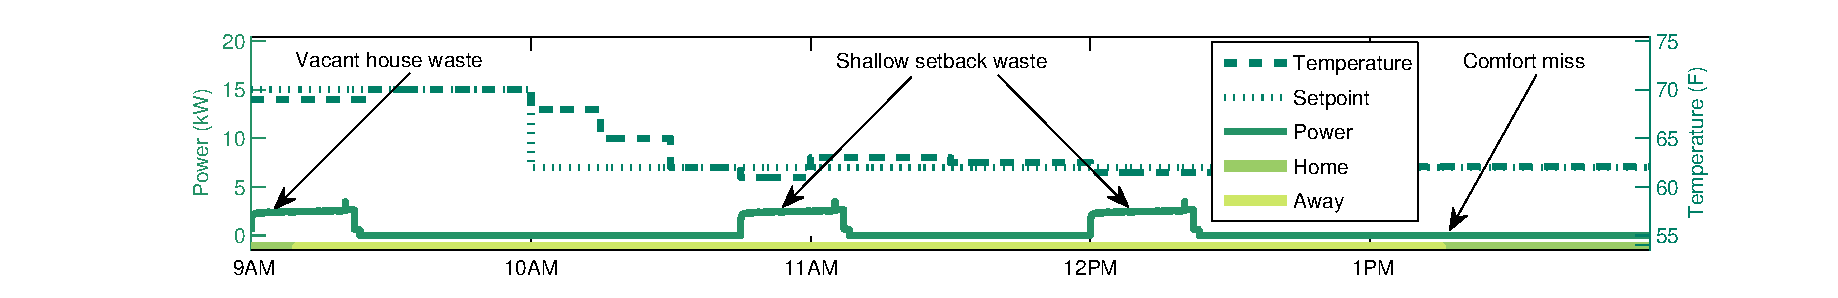
\includegraphics[width=1\columnwidth]{fig/scheduled}
} \caption[Drawbacks of Programmable Thermostats]{Programmable thermostats cause substantial energy waste and
  discomfort.} 
\label{fig:overviewScheduled}
\end{figure*}
%------------------------------------------------------------------------------
  
Programmable thermostats operate on a pre-defined {\em setback schedule}: the
house is conditioned to a {\em setpoint} temperature when the occupants are
typically active, and floats to a more energy efficient {\em setback}
temperature when the occupants are typically away or asleep. This approach
wastes energy in several ways, as illustrated by the composite of data traces in
Figure~\ref{fig:overviewScheduled} that were collected from a home using a
programmable thermostat. First, the occupants leave the home shortly after 9am,
but the system wastes energy because it is scheduled to continue heating the
home until 10am (left side). Second, the setback temperature is well above
safety limit for a home, causing energy consumption even while the house is
vacant (center). This type of {\em shallow setback} is typically used as a
safety precaution, in case the building actually is occupied at that
time. Third, the occupants become uncomfortable when they return shortly after 1
pm because the system is not scheduled to heat the house until much later. This
causes people to reduce their use of setback schedules, or stop using them
altogether. Over 50\% of households that have programmable thermostats are
reported to not use setback periods at night or during the
day~\cite{sumfindings}. In contrast, households with the simpler dial-type
thermostats can easily adjust temperature settings before going to sleep or
leaving the house, and as a result actually save more energy on average than
households with programmable thermostats\cite{sumfindings, sachs04}.

\subsubsection{Reactive Thermostats}

Reactive thermostats use heating, or cooling, patterns to ensure that a home
reaches a comfortable setpoint when occupied. They learn the residents'
temperature preferences~\cite{keyson2000intelligent}, use sensors to infer
occupancy patterns~\cite{fountain1994comport}, or use light
levels~\cite{titus1996advanced} to determine when to change setpoints or airflow
through the house~\cite{fujii1992japanese}. The complexity associated with these
thermostats means that any miscalculations, or errors in models used, could lead
to energy wastage or discomfort to occupants. In
Section~\ref{sec:occupancyOrientedHVACControl}, we present a few reactive
thermostats that use occupancy to control HVAC systems.

\subsection{Occupant-Oriented HVAC Control} 
\label{sec:occupantOrientedHVACControl}
%------------------------------------------------------------------------------
% Figure 1
\begin{figure*}[t]
\centering{
  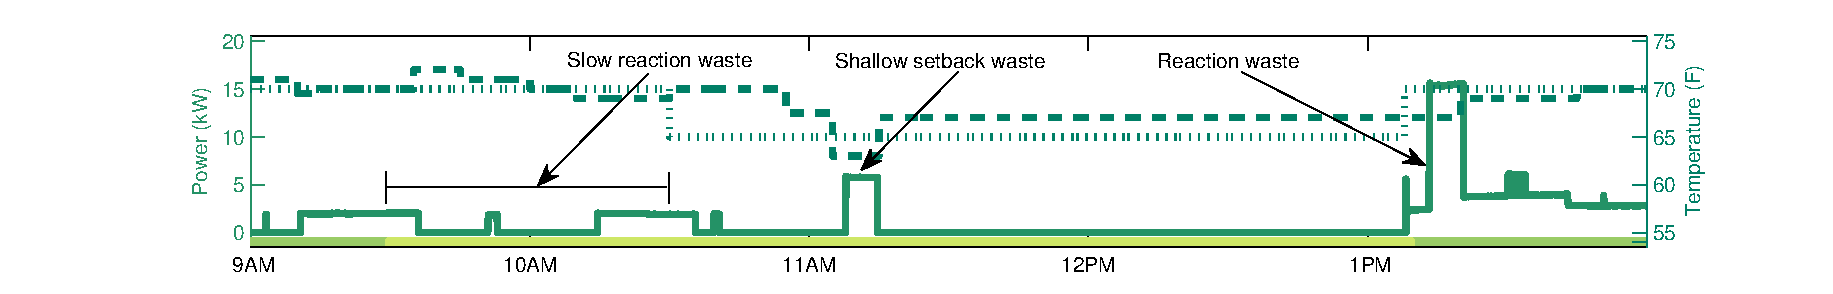
\includegraphics[width=1\columnwidth]{fig/reactive}
} \caption[Drawbacks of Occupant-oriented Thermostats]{Occupant-oriented thermostats have three sources of energy waste.} 
\label{fig:overviewReactive}
\end{figure*}
%------------------------------------------------------------------------------

Thermostatic control wastes energy due to occupancy patterns varying from the
pre-defined schedule, and the system having to maintain a setback temperature
close to the setpoint temperature so as to minimize discomfort if the occupants
become active unexpectedly (Figure~\ref{fig:overviewReactive}). In order to
remove the burden of having the program a thermostat based on occupancy
patterns, the {\em self-programming thermostat} which automatically chooses the
optimal setback schedule was proposed~\cite{gao2009self}. This system does not
fully solve the problems because occupancy patterns change every day, and so
{\em any} static schedule must either waste energy or sacrifice occupant
comfort.

As an extension to this method, we implemented {\em Smart Thermostat} which
incorporated dynamic actuation in order to minimize the energy wastage and loss
of comfort due to variations in occupancy patterns~\cite{Lu2010}. We used data
collected from eight homes over a period of two weeks to train a Hidden Markov
Model (HMM) using leave-one-out cross-validation. This model was used to predict
occupancy and control a mult-stage HVAC system. While this approach goes a long
way in minimizing the energy consumed by not conditioning an unoccupied house,
there is still a lot of savings to be had by not conditioning unoccupied spaces
of an occupied house.

Gupta et al.~\cite{gupta2009adding} add GPS-control to traditional thermostats
by using information from location aware mobile phones to augment thermostats
with the ability to control HVAC systems using travel time. By estimating how
long it takes for the residents to return to an unoccupied home, the thermostat
can be placed in a ``just-in-time'' travel-to-home-time mode so that it starts
conditioning the house in time for the residents' arrival, thus staying in a
lower-power setback mode for longer. Through simulations, the authors
demonstrate energy savings of up-to 7\% in certain households. While this system
is one solution to the problem of efficiently using programmable thermostats, it
generally results in lower savings than programmable or manual thermostats and
does not provide any energy savings in heating or cooling occupied houses.

Mozer et al. present the {\em Neurothermostat} which uses daily occupancy
schedules and a neural network trained on five months of occupancy data in order
to control an HVAC system~\cite{mozer1997neurothermostat}. The authors
demonstrate that the Neurothermostat results in a lower unified cost, defined as
a combination of energy usage and occupant discomfort. Similarly, Scott et
al. implemented {\em PreHeat}~\cite{scott2011preheat} which uses occupancy
sensing and occupancy prediction to automatically control home heating. The
system was implemented in three homes in the United States and two homes in the
United Kingdom. Leveraging the room-level radiators and underfloor heating units
commonly used in the UK, PreHeat provided room-level heating control. Occupancy
was detected using RFID tags placed on the house keys do sense if the house was
occupied or vacant and motion sensors in each room, in the UK houses, to detect
if rooms were occupied. While PreHeat demonstrates the energy saving potential
of occupant-oriented room-level heating control, it does so with only
independent room-level heating units. Even though the authors implemented the
system in three US houses with central heating systems, they resorted to
whole-house occupancy-based control due to the difficulties of implementing
room-level control with an existing centralized HVAC system. We provide
solutions to enable such a retrofit to the many homes in the United States that
have centralized HVAC systems.

Some commercial buildings are beginning to use occupancy sensors to create a
tighter link between occupancy and HVAC control with reactive thermostats that
use motion, window, and/or door sensors to turn the HVAC system on or off after
detecting that the occupants have left or returned to a space. For example, the
Telkonet SmartEnergy~\cite{telkonet} control system allows the user to define a
maximum recovery time parameter, which is set by the user. When the space is
unoccupied, the system maintains a setback temperature from which it can return
to the setpoint within the specified recovery time, once the occupants
return. The system estimates the response time based on building and system
parameters as well as current weather conditions. Other similar commercial
systems include the Verdant~\cite{prothermostats}, Viconics~\cite{vt7000}, and
PECO~\cite{peco} systems. While reactive thermostats are a step in the right
direction, they are almost always applied to hotel rooms because they rely on
the simplicity of hotel rooms and the keyed entrance to identify occupants; more
complex spaces with multiple rooms, entrances, and occupants require more
advanced sensing technology, such as the techniques discussed in this proposal.

\subsection{Room-Level Zoning} 
Traditional zoned HVAC systems separate a house into zones by floor with the
floor where the bedrooms are located being conditioned at night while the floor
with the living areas being conditioned during the day. Such systems have
resulted in homeowners saving as much as 20-30\% as compared to single zoned
systems~\cite{Systems2003}. Such systems have to be installed when the house is
built or requires extensive modifications to the HVAC system which most
homeowners will not be willing to undertake. Previous researchers have
investigated using multiple temperature sensors in a building with a single
thermostat~\cite{lin2002multi}. This work, done in simulation, demonstrated an
increase in user comfort by using targeted comfort control strategies. Others
retrofitted a house in Danville, CA with wirelessly controllable registers and
demonstrated that energy savings is possible by directed air into localized
zones~\cite{watts2007application}. This work did not use occupant information to
control the HVAC system.

State of the art multiple zone wireless HVAC control systems are also available
for commercial buildings. Discharge-air-regulation technique (DART), implements
wireless mesh networking to measure temperature and control HVAC fan
speed~\cite{federspiel2006wireless}. Millennial Net~\cite{Net2009} and Siemens
APOGEE~\cite{Inc.2010} offer wireless solutions to building control and
measurement. The latter systems utilize wireless temperature nodes but the HVAC
controls are wired to the thermostat control system. Just like the residential
zoning systems, these multiple zone solutions often require expensive
retrofits. This proposal focuses on a more cost effective alternative by
automating vent registers rather than altering the entire HVAC system. With
wirelessly controlled louvers, a low cost software based home controller would
be able to increase comfort and save energy by closing off vents to areas where
conditioning is not needed~\cite{redfern2006design}.

Since not all the rooms on a particular floor are used during a particular
period of time, energy is wasted in conditioning these unoccupied
rooms. Numerous studies have shown that providing individual temperature control
in rooms provide increased comfort for the occupants in addition to energy
savings~\cite{Airgonomix2008}. 

As the premier organization for national green building guidelines,
USGBC~\cite{Council} formulated the LEED (Leadership in Energy and Environmental
Design) green building criteria to rate and recognize energy efficient
buildings. According to USGBC, efficient HVAC systems can reduce up to 60\% of
energy costs related to heating and cooling a building. USGBC's energy
efficiency guidelines for HVAC systems include:
\begin{itemize}
\item Engineering for dynamic thermal zone sizing
\item Engineering for individual control of thermal conditions
\end{itemize}
Buildings that install equipment and follow practices that support those two
guidelines, earn credit that go towards achieving a specific LEED designation
such as Silver, Gold, or Platinum. Sub-zoning supports both of the LEED
guidelines listed above~\cite{Loftness2003}. 

Rose et al. studied various HVAC system controls for the Environmental
Protection Agency, some of which allowed for control over individual rooms. The
analyzed sub-zoned systems reported energy savings of 43\% compared to
conventional zoned HVAC systems~\cite{rose1997epa}. A report prepared for TIAX,
a company that specialized in bringing new inventions and technologies to
market, found potential energy savings of 0.07 quads (or $7*10^{13}$ BTU) across
the entire U.S. office market with zub-zoned HVAC
technology~\cite{llc2002energy}. This is enough to power the entire state of New
York for a week~\cite{EIA2008}. Moreover, the system tested used additional fans
to redirect airflow, adding equipment and operational cost. Without these costs,
even more energy could be saved. 

